\chapter{Why MEU?}\label{ch:risk}

\section{Arguments for the MEU Principle}\label{sec:why-meu}

So far, we have largely taken for granted that rational agents maximize expected
utility. It is time to put this assumption under scrutiny.

In chapter \ref{ch:overview}, I gave a simple initial argument for the MEU
Principle. An adequate decision rule, I said, should consider all the outcomes
an act might bring about -- not just the best, the worst, or the most likely --
and that it should weigh outcomes in proportion to their probability, so that
more likely outcomes are given proportionally greater weight.

In chapter \ref{ch:utility}, we looked at the internal structure of utility. I
didn't mention it at the time, but the account we developed can be used to
support the MEU Principle.

Consider a schematic decision matrix with $n$ states $S_{1},\ldots,S_{n}$. The
expected utility of an act $A$ is
\[
  \EU(A) = \U(O_{1})\cdot \Cr(S_{1}) + \ldots + \U(O_{n})\cdot \Cr(S_{n}).
\]
In an adequate decision matrix, any act $A$ in conjunction with any state
$S_{i}$ should determine the relevant outcome $O_{i}$, so that $S_{i} \land A$
entails $O_{i}$. Since outcomes have uniform utility, it follows that
$\U(A \land S_{i}) = \U(O_{i})$, for all $i$. Thus
\[
  \EU(A) = \U(A \land S_{i})\cdot \Cr(S_{1}) + \ldots + \U(A \land S_{n})\cdot \Cr(S_{n}).
\]

In an adequate decision matrix, the states are independent of the acts. This suggests that $\Cr(S_{i} / A) = \Cr(S_{i})$. So
\[
  \EU(A) = \U(A \land S_{i})\cdot \Cr(S_{1}/A) + \ldots + \U(A \land S_{n})\cdot \Cr(S_{n}/A).
\]

In section \ref{sec:structure-of-utility}, I mentioned a ``partition
formulation'' of Jeffrey's axiom. This says that for any proposition $A$ and
partition $S_{1},\ldots,S_{n}$,
\[
  \U(A) = \U(A \land S_{1})\cdot \Cr(S_{1}/A) + \ldots + \U(A \land S_{n})\cdot \Cr(S_{n}/A).
\]
Since the states in a decision matrix form a partition, it follows that
$\EU(A) = \U(A)$: the \emph{expected utility} of an act equals its
\emph{utility}.

It might seem strange to speak of an act's utility. When we use the MEU
Principle, we assign \emph{utilities} to outcomes and \emph{expected utilities}
to acts. We never talk about the utility of an act. In the terminology of
chapter \ref{ch:utility}, each outcome is a ``concern'', as it settles
everything the agent cares about. The theory of utility that we developed in
chapter \ref{ch:utility} allows us to extend an agent's ``intrinsic'' utility
function for concerns to other propositions. In particular, we can talk about
the utility of propositions that specify an act.

An act's utility measures how strongly the agent desires to perform the act.
Assuming the theory of utility from chapter \ref{ch:utility}, the MEU principle
reduces to the seemingly innocuous claim that rational agents choose an act that
they desire to perform at least as strongly as any alternative. (We are going to
challenge this seemingly innocuous claim in chapter \ref{ch:cdt}.)

In chapter \ref{ch:preference}, we met yet another argument for the MEU
Principle. The argument began with an idea about how to measure (or define) an
agent's intrinsic utility function. The idea was to look at the agent's
preferences between outcomes and lotteries. Assuming that the agent always
chooses a most preferred option, von Neumann's construction of utility entails
that an agent obeys the MEU Principle (in choices between lotteries) iff their
preferences satisfy certain ``axioms'': Transitivity, Completeness, Continuity,
Independence, and Reduction.

% Should we pause to think about the assumption that rational agents always
% choose a most preferred option, given the earlier discussion about the
% connection between preference and choice?

To complete this argument for the MEU Principle (for choices between lotteries),
we would need to explain why the axioms should be considered requirements of
rationality. Why should rational preferences satisfy Transitivity, Completeness,
Continuity, Independence, and Reduction?

Here is an attractive answer: if an agent violates these axioms, then they will
make patently bad choices in certain multi-stage decision problems.

To illustrate, suppose your preferences violate the Transitivity axiom. You
prefer $A$ to $B$, $B$ to $C$, but $C$ to $A$. Your preferences form a cycle.
Whichever of $A$, $B$ or $C$ you have, you would prefer to have one of the
others. If you are willing to pay a small amount to get the preferred option, it
looks like I could exploit you in a kind of multi-stage Dutch Book.

Concretely, let's assume you start out with $C$. Since you prefer $B$ to $C$,
you should be willing to pay an insignificant amount (say, 1p) if I let you swap
$C$ for $B$. Once you have $B$, I let you swap $B$ for $A$ in exchange for
another penny. You should be happy to do that, given that you prefer $A$ to $B$.
Finally, I let you swap $A$ for $C$, again in exchange for 1p. You should
accept, as you prefer $C$ to $A$. You are back where you started, with $C$, and
I have gained three pence. We could start over, letting you swap $C$ for $B$ for
$A$ for $C$ until I have emptied your wallet.

This kind of argument is called a \textbf{money-pump argument} (for obvious
reasons). It's worth spelling out in more detail. In its present form, the
argument has a serious flaw.

\section{Money pumps and sequential choice}\label{sec:sequentialchoice}

We are looking at an agent with cyclical preferences:
\begin{gather*}
  A \pref B\\
  B \pref C\\
  C \pref A
\end{gather*}
We imagine presenting this agent (``you'') with a sequence of choices. A
decision problem with more than one choice is called a \textbf{sequential
  decision problem}. The branch of decision theory that studies sequential
decision problems is called \textbf{sequential decision theory} or
\textbf{dynamic decision theory}. Our money-pump argument invites us to take a
brief look into this area.

We have assumed that you start with $C$. At the first choice point in our
money-pump scenario, you can either keep $C$ or exchange $C$ for $B$, at a small
cost. Let $B^{\text{-}}$ express $B$ with the added small cost:
$B^{\text{-}} = B \land $-1p. So your first choice is between $C$ and
$B^{\text{-}}$. If you choose $B^{\text{-}}$, you get the option to pay another
penny to swap $B$ for $A$. If you accept, you are left with
$A^{\text{-}\text{-}}$ = $A \land$-2p. You are then offered a third choice, in
which you can stick with $A^{\text{-}\text{-}}$ or end up with
$C^{\text{-}\text{-}\text{-}} = C \land$-3p.

We can picture the whole sequential decision problem in a tree diagram, called
an \textbf{extensive form representation}.

\begin{center}
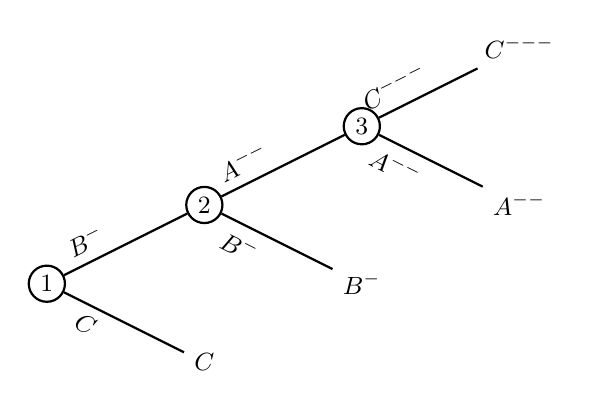
\begin{tikzpicture}[thick,
    circ/.style={circle,draw,thick,inner sep=2pt,font=\small},
    end/.style={font=\small},
    leftlabel/.style={above,sloped,near start,font=\small},
    rightlabel/.style={below,sloped,near start,font=\small},
    every label/.style={font=\small}]
  \node[circ] (1) at (0,0) {1}; % node (1)
  \node[circ] (2) at (2,1) {2}; % node (2)
  \node[end] (C) at (2,-1) {$C$}; % end node: C
  \draw (1) -- node[leftlabel] {$B^{\text{-}}$} (2); % line (1) -> (2)
  \draw (1) -- node[rightlabel] {$C$} (C); % line (1) -> C
  \node[circ] (3) at (4,2) {3}; % node (3)
  \node[end] (BM) at (4,0) {$B^{\text{-}}$}; % end node: B-
  \draw (2) -- node[leftlabel] {$A^{\text{-}\text{-}}$} (3); % line (2) -> (3)
  \draw (2) -- node[rightlabel] {$B^{\text{-}}$} (BM); % line (2) -> B-
  \node[end] (CM) at (6,3) {$C^{\text{-}\text{-}\text{-}}$}; % end node: C-
  \node[end] (AMM) at (6,1) {$A^{\text{-}\text{-}}$}; % end node: A--
  \draw (3) -- node[leftlabel] {$C^{\text{-}\text{-}\text{-}}$} (CM); % line (3) -> C-
  \draw (3) -- node[rightlabel] {$A^{\text{-}\text{-}}$} (AMM); % line (3) -> A--
\end{tikzpicture}
\end{center}

The circled nodes are choice points. What path through this tree would you take?

Above, I assumed that you would choose $B^{\text{-}}$ at node 1. My reasoning
was that you prefer $B$ to $C$, and we take for granted that the preference is
strong enough that you also prefer $B^{\text{-}}$ to $C$. For analogous reasons,
I assumed that you would choose $A^{\text{-}\text{-}}$ at node 2 (because you
prefer $A$ to $B$), and $C^{\text{-}\text{-}\text{-}}$ at node 3 (because you
prefer $C$ to $A$). You end up with $C^{\text{-}\text{-}\text{-}} = C \land $-3p,
even though you could have gotten $C$ at no cost by ``turning right'' at the
first node.

But would you really make these choices?

Look again at node 1. Superficially, you are here offered a choice between $C$
and $B^{\text{-}}$. But if you ``choose $B^{\text{-}}$'' you aren't actually
getting $B^{\text{-}}$ unless you ``turn right'' at node 2. If you turn left at
node 2 and again at node 3, as we assumed you will, then ``choosing
$B^{\text{-}}$'' at node 1 actually means getting
$C^{\text{-}\text{-}\text{-}}$. And $C^{\text{-}\text{-}\text{-}}$ is worse than
$C$. If you can foresee that you will turn left at nodes 2 and 3, then you will
\emph{not} turn left at node 1.

The flaw in my argument is that I have ignored any information you might have
about your predicament and about what you might do at later stages in the
scenario. We have adopted what is called a \textbf{myopic} approach to
sequential choice. The myopic approach treats each choice as if it were the only
decision the agent ever faces, ignoring any downstream consequences. We
shouldn't be myopic. An adequate evaluation of the agent's options should take
into account what the agent is likely to do later. This approach to sequential
choice is called \textbf{sophisticated}.

To investigate our decision problem from a sophisticated perspective, we need to
say what you know about your situation. Let's assume that you are fully
informed about the sequential decision problem. Let's also assume that you have
perfect knowledge of your preferences, so that you can figure out what you will
do at any future choice point.

What you should do at node 1 now depends on what you might do at node 2, which
similarly depends on what you might do at node 3. But if there are no relevant
choices after node 3 then we can figure out what you would do here. The choice
at node 3 is between $A^{\text{-}\text{-}}$ and $C^{\text{-}\text{-}\text{-}}$.
Since you prefer $C$ to $A$, it is plausible that you will choose
$C^{\text{-}\text{-}\text{-}}$.

% Although note that we here assume a naive connection between preference and
% choice.

With this information in hand, we can return to node 2. Your choice at node 2 is
effectively between $C^{\text{-}\text{-}\text{-}}$ (\emph{via} node 3) and
$B^{\text{-}}$. You prefer $B$ to $C$. So we can expect you to choose
$B^{\text{-}}$ at node 2.

Now return to node 1. Given what we have just figured out, the choice at node 1
is effectively between $C$ and $B^{\text{-}}$. You prefer $B$ (and
$B^{\text{-}}$) to $C$. We may therefore expect you to choose $B^{\text{-}}$ at
node 1. You will ``turn left'' at node 1 and right at node 2.

This kind of reasoning is called \textbf{backward induction}. We'll meet it
again in section \ref{sec:sequentialgames}, where we will see that it is not as
harmless at it might appear.

\begin{exercise}{3}
  Draw a decision matrix (without utilities) for your choice at node 1.
\end{exercise}

The money pump argument from the previous section doesn't work -- at least not
if you know about my plot. But this can be fixed. In the following sequential
decision problem, an agent who prefers $A$ to $B$ to $C$ to $A$ would trade $A$
for $A^{\text{-}}$ at node 1, assuming they know about the scenario and their
preferences. They would make a guaranteed and avoidable loss of 1 penny.

\begin{center}
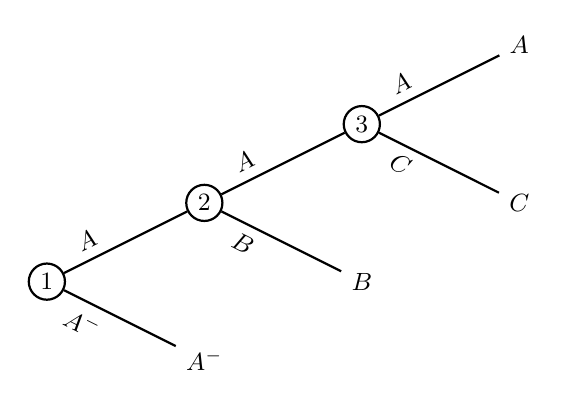
\begin{tikzpicture}[thick,
    circ/.style={circle,draw,thick,inner sep=2pt,font=\small},
    end/.style={font=\small},
    leftlabel/.style={above,sloped,near start,font=\small},
    rightlabel/.style={below,sloped,near start,font=\small},
    every label/.style={font=\small}]
  \node[circ] (1) at (0,0) {1}; % node (1)
  \node[circ] (2) at (2,1) {2}; % node (2)
  \node[end] (AM) at (2,-1) {$A^{\text{-}}$}; % end node: A-
  \draw (1) -- node[leftlabel] {$A$} (2); % line (1) -> (2)
  \draw (1) -- node[rightlabel] {$A^{\text{-}}$} (AM); % line (1) -> A-
  \node[circ] (3) at (4,2) {3}; % node (3)
  \node[end] (BM) at (4,0) {$B$}; % end node: B
  \draw (2) -- node[leftlabel] {$A$} (3); % line (2) -> (3)
  \draw (2) -- node[rightlabel] {$B$} (BM); % line (2) -> B
  \node[end] (AM) at (6,3) {$A$}; % end node: C
  \node[end] (CMM) at (6,1) {$C$}; % end node: A
  \draw (3) -- node[leftlabel] {$A$} (AM); % line (3) -> A
  \draw (3) -- node[rightlabel] {$C$} (CMM); % line (3) -> C
\end{tikzpicture}
\end{center}

\begin{exercise}{2}
  Explain by backward induction why ``you'' (the agent with cyclical
  preferences) would choose $A^{\text{-}}$ at node 1.
\end{exercise}
\begin{exercise}{1}
  Which choices would you make at which nodes if your preferences were
  transitive, so that $A \pref B$, $B \pref C$, and $A \pref C$?
\end{exercise}

The real point is, of course, not about money. The point is that cyclical
preferences effectively lead to the choice of a dominated strategy. You could
have gotten $A$, by ``turning left'' at each node. Due to your cyclical
preferences, you end up with a strictly worse outcome $A^{\text{-}}$.

We have assumed that you prefer $A$ to $B$, $B$ to $C$, and $C$ to $A$. Not all
violations of Transitivity involve cycles of this kind. Instead of preferring
$C$ to $A$, you could be indifferent between $C$ and $A$. You could also have no
attitude at all about the comparison between $A$ and $C$, violating both
Transitivity and Completeness. These preferences, too, can be shown to support
the choice of a dominated strategy. The same is true, more generally, for
(almost) all preferences that violate the von Neumann and Morgenstern axioms.

% Needless to say, the arguments have not gone unchallenged. Some hold it is
% simply not a sign of irrationality that an agent gets a worse outcome in a
% sequential decision problem than they could have gotten by choosing a different
% path through the tree. Some hold that if an agent knows that she is facing a
% sequential decision problem, then she should simply choose a path and stick to
% it, no matter if the individual choices are in line with her preferences.
% Finally, note that our argument presupposes that the same outcome $A$ may occur
% at multiple points in a decision tree. We will soon find reasons to doubt this.

% Note also that our argument relies on a naive assumption about the connection
% between preference and choice


\section{The long run}

I want to look at one more argument for the MEU Principle. This one turns on a
connection between probability and relative frequency.

Suppose you repeatedly toss a fair coin, keeping track of the number of heads
and tails. You will find that over time, the proportion of heads approaches its
objective probability, $\nicefrac{1}{2}$. After one toss, you will have 100\%
heads or 100\% tails. After ten tosses, it's very unlikely that you'll still
have 100\% heads or 100\% tails. 60\% heads and 40\% tails wouldn't be unusual.
The (objective) probability of getting 40\% tails or less in 10 independent
tosses of a coin is 0.377. For 100 tosses, it is 0.028; for 1000, it is less
than 0.000001. After 1000 tosses, the probability that the proportion of tails
lies between 45\% and 55\% is 0.999.

In general, the rules of probability entail that if there is a sequence of
``trials'' $T_1,T_2,T_3\ldots$ in which the same outcomes (like heads and tails)
can occur with the same probabilities, then the probability that the
\emph{proportion} of any outcome in the sequence differs from its
\emph{probability} by more than an arbitrarily small amount $\epsilon$ converges
to 0 as the number of trials gets larger and larger. This is known as the
\textbf{(weak) law of large numbers}. Loosely speaking: in the long run,
probabilities turn into proportions.

How is this relevant to the MEU Principle? Consider a bet on a fair coin flip:
if the coin lands heads, you get £1, otherwise you get £0. The bet costs £0.40.
If you are offered this deal again and again, the law of large numbers entails
that the percentage of heads will (with high probability) converge to 50\%. If
you buy the bet each time, you can be confident that you will loose £0.40 in
about half the trials and win £0.60 in the other half. The £0.10 \emph{expected
  payoff} turns into an \emph{average payoff}. In this kind of scenario, the MEU
Principle effectively says that you should prefer acts with greater average
utility (and therefore greater total utility) over acts with lower average (and
total) utility. If you face the same decision problem over and over, then you
are almost certain to achieve greater total utility if you follow the MEU
Principle than if you follow any other rule.

In reality, of course, there are limits to how often one can encounter the very
same decision problem. ``In the long run, we are all dead'', as John Maynard
Keynes quipped. Fortunately, we saw in the coin flip example that the
convergence of proportions to probabilities tends to be quick. It does not take
millions of tosses until the percentage of heads is almost certain to exceed
40\%.

As it stands, the long-run argument still assumes that the same decision problem
is faced over and over. But we can weaken this assumption. Suppose you face a
sequence of decision problems that may involve different outcomes, different
states, and different probabilities. One can show that if the states in these
problems are probabilistically independent, and the relevant probabilities and
utilities are not too extreme, then over time, maximizing expected utility is
likely to maximize average (and total) utility.

% \begin{exercise}
%   If you play roulette in a casino, the possible outcomes vary wildly:
%   you might lose a lot or you might win even more. Nonetheless,
%   roulette operators have fairly stable income streams and almost
%   never run out of money. How is that possible?  $\star$
% \end{exercise}

From all this, you might expect that professional gamblers and investors
generally put their money on the options with greatest expected payoff, since
this would give them the greatest overall profit in the long run. But they do
not. (Those who do don't remain professional gamblers or investors for long.)
To see why, imagine you are offered an investment in a startup that tries to
find a cure for snoring. If the startup succeeds, your investment will pay back
tenfold. If the startup fails, the investment is lost. The chance of success is
20\%, so the expected return is $0.2 \cdot 1000\% + 0.8 \cdot 0\% = 200\%$. Even
if this exceeds the expected return of all other investment possibilities, you
would be mad to put all your money into this gamble. If you repeatedly face this
kind of decision and go all-in each time, then after ten rounds you are bankrupt
with a probability of $1-0.2^{10} = 0.9999998976$.%
\cmnt{%
  (With the remaining 0.0000001024 probability your wealth would have increased
  1,000,000,000,000\%.)%
} %

This does not contradict the law of large numbers. In the startup example, you
are not facing the same decision problem again and again. If you lose all your
money in the first round, you don't have anything left to invest in later
rounds. Still, the example illustrates that by maximizing expected utility you
don't always make it likely that you will maximize average or total utility in
the long run. More importantly, the example suggests that there is something
wrong with the MEU Principle. Sensible investors balance expected returns and
risks. A safe investment with lower expected returns is often preferred to a
risky investment with greater expected returns. Shouldn't we adjust the MEU
Principle, so that agents can factor in the riskiness of their options?

\begin{exercise}{2}
  Every year, an investor is given £100,000, which she can either invest
  in a risky startup of the kind described (a different one
  each year), or put in a bank account at 0\% interest. If she always
  chooses the second option, she will have £1,000,000 after ten years.
  \begin{enumerate}
  \item[(a)] What are the chances that she would do at least as well
    (after ten years) if she always chooses the first option, without
    reinvesting previous profits?
    %(Hint: Compute the chance that she would do worse.)
  \item[(b)] How does the answer to (a) mesh with my claim in the text
    that an investor who always goes with the risky option is
    virtually guaranteed to go bankrupt?
  \end{enumerate}
\end{exercise}

\section{Risk aversion}

\cmnt{%
  Taleb: ```Psychologists determine our “paranoia” or “risk aversion” by
  subjecting a person to a single experiment -- then declare that humans are
  rationally challenged as there is an innate tendency to “overestimate” small
  probabilities. It is as if the person will never again take any personal tail
  risk! Recall that academics in social science are ... dynamically challenged.
  Nobody could see the grandmother-obvious inconsistency of such behavior with
  our ingrained daily life logic. Smoking a single cigarette is extremely
  benign, so a cost-benefit analysis would deem one irrational to give up so
  much pleasure for so little risk! The flaw in psychology papers is to believe
  that the subject doesn’t take any other tail risks anywhere outside the
  experiment and will never take tail risks again. ... our wiring might be
  adapted to “say no” to tail risk.'''
} %

Many people are risk averse, at least for certain kinds of choices. They prefer
situations with a predictable outcome over highly unpredictable situations. This
does not seem irrational. Does it pose a threat to the MEU Principle?

A standard way to measure risk aversion involves lotteries. Consider a lottery
with an 80\% chance of £0 and a 20\% chance of £1000. The expected payoff is
£200. Given a choice between the lottery and £100 for sure, a risk averse agent
might prefer the £100. Can we account for these preferences?

We can. We could, for example, assume that the difference in utility between
£1000 and £100 is, for this agent, less than five times the difference in
utility between £100 and £0. For example, if $\U(\text{£0}) = 0$,
$\U(\text{£100}) = 1$, and $\U(\text{£1000}) = 4$, then the lottery has expected
utility $0.8 \cdot 0 + 0.2 \cdot 4 = 0.8$, which is less than the guaranteed
utility of the £100.

This is how economists model risk aversion. They assume that for risk averse agents,
utility is a ``concave function of money'', meaning that the amount
of utility that an extra £100 would add to an outcome of £1000 is less than the
amount of utility the same £100 would add to a lesser outcome of, say, £100. We
have already encountered this phenomenon in chapter \ref{ch:utility}, where we
saw that money has declining marginal utility: the more you have, the less
utility you get from an extra £100. According to standard economics, risk
aversion is the flip side of declining marginal utility.

This should seem strange. Intuitively, the fact that the same amount of money
becomes less valuable the more money you already have has nothing to do with risk.
Money could have declining marginal utility even for an agent who loves the
thrill of risky options. Conversely, an agent might value every penny as much as
the previous one, but shy away from risks.

% The problem is that risk neutrality combined with declining marginal
% utility seems to support the exact same choices as risk aversion
% combined with non-declining marginal utility. So if an agent's utility
% function is defined through her preferences or choice dispositions
% over monetary gambles -- by the von Neumann and Morgenstern method,
% perhaps -- then the intuitive difference between risk aversion and
% declining marginal utility collapses.

% You can spin this both ways. You can conclude that we should reject
% the intuitive difference between risk aversion and declining marginal
% utility. Or you can hold on to the intuitive difference and conclude that
% utilities cannot be defined through preferences over monetary gambles.

No doubt some actions that appear to display risk aversion (say, among
professional gamblers) are really explained by the declining marginal utility of
money. But many people prefer predictable situations in a way
that can't be explained along these lines. The following example is due to
Maurice Allais,

\begin{example}(Allais's Paradox)[label=ex:allais]
  A ball is drawn from an urn containing 80 red balls, 19 green balls,
  and 1 blue ball. Consider first a choice between the following two
  lotteries. Which do you prefer?
  \vspace{-5mm}

  \begin{dmatrix}{c|c|c|c}\hline
     & Red {\small(0.8)} & Green {\small(0.19)} & Blue {\small(0.01)}\\\hline
     $A$ & £0 & £1000 & £1000 \\\hline
     $B$ & £0 & £1200 & £0  \\\hline
  \end{dmatrix}
  \vspace{-2mm}

  Next, consider the alternative lotteries $C$ and $D$, based on the
  same draw from the urn. Which of these do you prefer?
 
  \vspace{-2mm}
  \begin{dmatrix}{c|c|c|c}\hline
     & Red {\small(0.8)} & Green {\small(0.19)} & Blue {\small(0.01)}\\\hline
    $C$ & £1000 & £1000 & £1000 \\\hline
    $D$ & £1000 & £1200 & £0 \\\hline
  \end{dmatrix}
  \vspace{-5mm}
\end{example}
%
If you choose $C$ in the second choice, you get £1000 for sure. If you choose
$D$, you get either £1000 (most likely) or £0 (least likely) or £1200. If you're
risk averse, it makes sense to take the sure £1000.

In the first choice, the most likely outcome is £0 no matter what you do. It may
seem reasonable to take the 19\% chance of getting £1200 (by choosing $B$)
rather than the 20\% chance of getting £1000 (by choosing $A$).

Many people, when confronted with Allais's puzzle, seem to reason in this way.
They prefer $C$ to $D$ and $B$ to $A$. These preferences can't be explained by
the declining marginal utility of money. Indeed, there is no way of assigning
utilities to monetary payoffs that makes a preference of $C$ over $D$ and $B$
over $A$ conform to the MEU Principle. If you have the risk averse preferences,
you appear to violate the MEU Principle.
% Since a risk averse agent may well have
% the preferences, genuine risk aversion does seem to pose a challenge to the MEU
% Principle.

\begin{exercise}{3}
  The preference for $C$ over $D$ and $B$ over $A$ appears to violate the
  Independence axiom of von Neumann and Morgenstern. Explain. (The axiom states
  that, for any $A, B, C$, if $A \succsim B$, and $L_1$ is a lottery
  that leads to $A$ with some probability $x$ and otherwise to $C$, and $L_2$ is
  a lottery that leads to $B$ with probability $x$ and otherwise to $C$, then
  $L_1 \succsim L_2$. You can assume Completeness.)
\end{exercise}

% We can be more specific. The risk-averse preferences appear to violate von
% Neumann's Independence axiom. To see this, let $L_1$ be a lottery that pays
% £1000 if a green or blue ball is drawn (otherwise £0), and let $L_2$ be a
% lottery that pays £1200 if a green ball is drawn (otherwise £0). In Allais's
% paradox, $A$ is (in effect) a lottery that leads to $L_1$ with probability 0.2
% and otherwise to £0. $B$ is a lottery that leads to $L_2$ with probability 0.2
% and otherwise to £0. The Independence condition therefore says that if
% $L_1 \succsim L_2$, then $A \succsim B$. By parallel reasoning with $C$ and $D$,
% we get:
% \begin{enumerate}
%   \itemsep0em 
% \item If $L_1 \succsim L_2$, then $A \succsim B$ and $C \succsim D$; and
% \item If $L_2 \succsim L_1$, then $B \succsim A$ and $D \succsim C$.
% \end{enumerate}
% No matter how you rank $L_1$ and $L_2$, you can't have $B \succ A$ and $C \succ D$.

% \begin{exercise}{2}
%   Does the preference of $B$ to $A$ and $C$ to $D$ violate strong separability
%   (across states), weak separability, or neither? (Explain briefly.)
% \end{exercise}

Some say that the kind of risk aversion that is manifested by a preference of
$B$ over $A$ and $C$ over $D$ is irrational. Rational agents, they say, can't
prefer predictable situations over unpredictable situations. This might be OK if
our topic were a special kind of ``economic rationality''. But it's not OK if
we're interested in a general model of how coherent beliefs and desires relate
to choice. There is nothing incoherent about a desire for predictability.

The following scenario, presented as a counterexample to the MEU Principle by
Mark J.\ Machina, reinforces this verdict.

\begin{example}[label=ex:diamond]
  A mother has a treat that she can give either to her daughter Abbie or to her
  son Ben. She considers three options: giving the treat to Abbie, giving it to
  Ben, and tossing a fair coin, so that Abbie gets the treat on heads and Ben on
  tails. Her decision problem might be summarized by the following matrix
  (assuming for simplicity that if the mother decides to give the treat directly
  to one of her children, she nonetheless tosses the coin, just for fun).
  %
  \vspace{-2mm}
\begin{dmatrix}{c|c|c}\hline
     & Heads & Tails \\\hline
    Give treat to Abbie ($A$) & Abbie gets treat & Abbie gets treat \\\hline
    Give treat to Ben ($B$) & Ben gets treat & Ben gets treat \\\hline
    Let the coin decide ($C$) & Abbie gets treat & Ben gets treat \\\hline
\end{dmatrix}
%
  \vspace{-1mm}
  \noindent
  The mother's preferences are $C \succ A$, $C \succ B$, $B \succ A$. % B > A because of the von Neumann discussion in the next section.
\end{example}

As in Allais's Paradox, there is no way of assigning utilities to the outcomes
in the decision matrix in example \ref{ex:diamond} that makes the mother's
preferences conform to the MEU Principle. Yet these preferences are surely not
irrational. The mother prefers $C$ because it is the most fair of the three
options. It would be absurd to claim that rational agents cannot value fairness.

% \begin{exercise}{3}
%   Which of the von Neumann and Morgenstern axioms do the mother's preferences
%   appear to violate? (Explain briefly.)
% \end{exercise}
% By Continuity, if $C \succ A$ and $A \sim B$, then there are lotteries between
% $C$ and $B$ that the agent regards as equivalent to $A$. But mom would strictly
% prefer any such lottery to $A$. Also a violation of independence.


\section{Redescribing the outcomes}

When confronted with an apparent counterexample to the MEU Principle, the first
thing to check is always whether the decision matrix has been set up correctly.
In particular, we need to check if the outcomes in the matrix specify everything
that matters to the agent.

% My matrices in example \ref{ex:allais} (Allais's Paradox) specify how much money
% you get depending on your choice and the draw. But if you're risk averse, then
% you don't just care about how much money you will have. You also care about
% risk. We need to add more information to the outcomes.

Consider the bottom right cell of the second matrix in example \ref{ex:allais}.
What will happen if you choose $D$ and the blue ball is drawn? You get £0. But
you might also feel frustrated about your bad luck: there was a 99\% chance of
getting at least £1000, and you got nothing! You probably don't like feeling
frustrated. If so, the feeling should be included in the outcome. The outcome in
the bottom right cell of the second matrix should say something like `£0 and
considerable frustration'.

By contrast, consider the bottom right cell in the first matrix. If you choose
$B$ and the blue ball is drawn, you get £0. The chance of getting £0 was
81\%, so you'll be much less frustrated about your bad luck.
% You may still regret not having taken $A$, but since $A$ was just as unsafe as
% $B$, you probably wouldn't think you made a terrible mistake.
The outcome in that cell might say something like `£0 and a little frustration'.
With these changes, the preference for $B$ over $A$ and $C$ over $D$ is easily
reconciled with the MEU Principle.

\begin{exercise}{1}
  Assign utilities to the outcomes in the two matrices, with the changes just
  described, so that $\EU(B) > \EU(A)$ and $\EU(C) > \EU(D)$.
\end{exercise}

Do these changes reflect the values of a risk averse agent? Arguably not. Just
as (genuine) risk aversion is not the same as declining marginal utility of
money, it is not the same as fear of frustration. Imagine you face Allais's
Paradox towards the end of your life. The ball will be drawn after your death,
and the money will go to your children. You will not be around to experience
frustration or regret. Nor might your children, if the whole process is kept
secret from them. But if you like predictable outcomes, you might still prefer
$B$ to $A$ and $C$ to $D$.

Let's ask again what will happen if you choose $D$ and the blue ball is drawn.
One thing that will happen is that you get £0. You may or may not experience
frustration and regret. But here's another thing that is guaranteed to happen.
You \emph{will have chosen a risky option instead of a safe (predictable)
  alternative}. If you are risk averse, then plausibly (indeed, obviously!) you
care about whether your choices are risky. So we should put that into the
outcome. The outcome should say something like `£0 and incurred avoidable risk'.

The outcome in the bottom right cell of the first matrix does not have the
second attribute, that you have incurred an avoidable risk. There is no safe
alternative in the first matrix. We can once again distinguish the two outcomes,
and reconcile your preferences with the MEU Principle.

\begin{exercise}{1}
  If you care about predictability and risk, then we should also distinguish the
  outcomes in all other cells of the matrix. Can you explain how?
\end{exercise}

% In general, the first strategy assumes that the ``attributes'' that make up an
% outcome are events that occur as a causal consequence of the relevant choice.
% Your frustration or regret might be such events. That you have chosen a risky
% option is not. This is not a separate event, caused by your choice of a risky
% option, as you can see from the fact that the ``occurrence'' of this event after
% your choice does not depend on the causal structure of the world.

% Let's say that an outcome is \textbf{individuated locally} if it only comprises
% causal consequences of the relevant choice. A locally individuated outcome
% entails nothing about what happened at or before the time of choice.
%
% All this is murky. If I just speak of causation, one might argue that an event
% like *being the first to climb Mt Everest* is caused by a decision to climb
% the mountain. I need to make sure the events are described intrinsically.

% One might define ``local'' as ``not sensitive to which alternatives were
% available''. In that sense, one might argue that fairness is local, but the
% kind of riskiness that is involved in the Allais preferences is not. But this
% isn't obvious. The greater riskiness of D than C could be explained without
% referring to their alternatives. Even more clearly, we could reward C by
% safety.

\begin{exercise}{1}[label=e:diamond]
  Redescribe the outcomes in example \ref{ex:diamond} so that the mother's
  preferences conform to the MEU Principle.
\end{exercise}

When social scientists discuss the MEU Principle, they generally assume that
utility is assigned to material goods (as I mentioned in section
\ref{sec:sources-utility}). On this approach, an outcome in a decision matrix
can only specify who owns which goods. Agents who care about frustration,
predictability, or fairness are said to violate the MEU Principle.

There are reasons for this restricted conception of utility. Assuming that
consumers maximise expected utility, in the restricted sense, and that material
goods have declining marginal utility, one can derive various ``laws'' of
microeconomics, such as the ``law of demand''. Even if people don't actually
maximise expected utility, in the restricted sense, their behaviour as consumers
might approximate what the economics version of our model predicts to make the
model theoretically useful.

But our goal is not to derive the laws of microeconomics from substantive
assumptions about what people ultimately care about. Our goal is to develop a
general model of belief, desire, and rational choice. In this context, we don't
want to put unnecessary and unrealistic constraints on what agents might desire.
We want to allow for agents who care about frustration, predictability,
fairness, and all sorts of other things.

Authors in the economics tradition sometimes consider models in which an agent's
choices are assumed to be determined by their desire towards material goods, as
reflected in their utility function, as well as their desire towards a specific
further attribute -- anticipated regret, for example, or riskiness. The MEU
Principle is then revised to make room for the further parameter besides the
agent's credence function and the utility function for material goods. But this
approach clearly doesn't generalise well. We have instead followed a popular
tradition in philosophy that puts no substantive constraints at all on the
objects of utility.

I should emphasize that these two approaches are not necessarily in tension. We
are simply engaged in different projects.

% But there is a lot of confusion. See e.g. Buchak's idea that utility measures
% the extent to which the agent desires the outcome ``in itself'', irrespective
% of its origin.

A common objection to our unrestrictive conception of utility is that it seems
to render the MEU Principle vacuous. In the economics interpretation, the MEU
Principle predicts that rational agents don't choose $B$ over $A$ and $C$ over
$D$ in Allais's Paradox. It also predicts that rational agents never toss a coin
to decide who gets a treat. Our MEU Principle makes no such predictions. Indeed,
for any pattern of behaviour, we can imagine that the agent has a basic desire
to display just that behaviour. Displaying the behaviour then evidently
maximizes expected utility. No behaviour whatsoever is, all by itself, ruled out
by our MEU Principle.

This isn't necessarily a problem -- not even for a descriptive understanding of
the principle. Many respectable scientific theories are unfalsifiable \emph{in
  isolation}. Scientific hypotheses can generally only be tested in conjunction
with a whole range of background assumptions.

The same is true for the MEU Principle, understood as a descriptive hypothesis
about human behaviour. \emph{Given} some assumptions about an agent's beliefs
and desires, we can easily find that their choices do not conform to the MEU
Principle. And we often have good evidence about the relevant beliefs and
desires. It is safe to assume that participants in the world chess
tournament want to win their games, and that they are aware of the current
position of the pieces in the game.

I said that any pattern of behaviour is compatible with the MEU Principle.
Didn't von Neumann and Morgenstern prove that an agent maximizes expected
utility in choices between lotteries \emph{if and only if} their preferences
(and therefore, one might think, their choice dispositions) satisfy some
non-trivial conditions -- Transitivity, Continuity, Independence, etc.?

Not quite. The proof of this result assumes that the agent's (intrinsic)
utilities are determined by von Neumann's method. And here we reach a genuine
downside to our approach: it breaks von Neumann's method.

Suppose, for example, we want to determine the intrinsic utility function for
the mother in example \ref{ex:diamond}. Let $a$ and $b$ be the outcomes of
directly giving the treat to Abby and to Ben, respectively. If the mother cares
about fairness, then one relevant aspect of both $a$ and $b$ is that the treat
is not allocated through a chance process. By von Neumann's method, we should
now ask whether the mother prefers some other outcome $c$ to a \emph{lottery $L$
  between $a$ and $b$}. This lottery would be a chance process that leads to
outcomes which don't come about through a chance process. That's logically
impossible. $L$ entails that one of $a$ and $b$ comes about, and it also entails
that neither of them come about. We can hardly assume that the mother has
interesting views about how $L$ compares to $c$.

In general, if we allow agents to care about arbitrary aspects of outcomes, then
we can't assume that any lottery between outcomes is logically possible. Either
the Completeness axiom or most of the other axioms become highly implausible.
% We either have a violation of completeness, if the agent doesn't have
% preferences involving impossible lotteries, or a violation of most other
% axioms, unless the agent prefers some impossible lotteries over others. Some
% authors, Buchak for example, seem to think that such hyperintensional
% preferences are OK.

This is a genuine cost. We lose a popular approach to defining utility, and a
popular argument for the MEU Principle.

\begin{exercise}{3}[label=e:nonlocalmoneypump]
  The money-pump argument for Transitivity from section
  \ref{sec:sequentialchoice} also makes substantive assumptions about what the
  agent (``you'') ultimately cares about. Explain.
\end{exercise}

Similar problems arise for other attempts to measure utility in terms of
preference, and to justify the MEU Principle. The popular theory of Leonard
Savage, for example, also assumes that an agent's utility function pertains to a
restricted set of ``outcomes'' that are logically independent of the ``states''
to which credences are assigned.

% Savage assumes that for any possible outcomes $a$ and $b$ and any state $S$,
% the agent has preferences concerning acts of the form $\bet{S}{a}{b}$. But if
% the agent is allowed to care about arbitrary attributes, then one of these
% attributes might well be (or entail) $S$. And if, say, $b$ entails $S$, then
% there can't be any act $\bet{S}{a}{b}$, for this would lead to $a$ if $S$ and
% to $b$ if $\neg S$.

Ramsey's approach, however, might still work. Remember that instead of
lotteries, Ramsey uses gambles of the form `$a$ if $N$, $b$ if $\neg N$', where
$N$ is some proposition the agent doesn't care about and $a$ and $b$ are among
the agent's concerns. If we understand such a gamble as a possible act that
leads to $a$ if $N$ and otherwise to $b$, then the gamble may become logically
impossible -- if, for example, $a$ entails that no such act is performed. But we
don't have to interpret gambles as hypothetical acts. A gamble could simply be a
certain kind of conditional proposition.

A clear example of a preference-based approach that imposes no substantive
constraints on basic desires was developed by Ethan Bolker and Richard Jeffrey
in the 1960s. Where von Neumann uses lotteries and Ramsey gambles, Bolker and
Jeffrey use unspecific propositions. If $a$ and $b$ are two concerns, then the
disjunction $a \lor b$ behaves somewhat like a lottery that ``leads to'' (i.e.,
amounts to) $a$ with some probability (credence) and to $b$ with another. As
long as $a$ and $b$ are consistent, $a \lor b$ is guaranteed to be consistent as
well.

Normally, the aim of a preference-based approach is to show that if an agent's
preferences satisfy some plausible conditions (``axioms''), then the preferences
can be represented by a utility function $\U$, perhaps together with a credence
function $\Cr$, relative to which the agent ranks the things over which the
preferences are defined by expected utility. Jeffrey and Bolker's preference
relation is defined over arbitrary propositions. It isn't clear how we should
understand the ``expected utility'' of, say, a disjunction $a \lor b$. But we've
seen above, in section \ref{sec:why-meu}, that Jeffrey's concept of utility,
which we have adopted since chapter \ref{ch:utility}, can be seen to generalise
the concept of expected utility. Jeffrey and Bolker show that if an agent's
preferences satisfy certain axioms, then the preferences can be represented by a
utility function $\U$ and a credence function $\Cr$ relative to which the agent
ranks propositions in line with Jeffrey's axiom.

So we might still be able to derive utility from preference -- although the
relevant preferences, relating arbitrary propositions, are even further removed
from choice dispositions than in von Neumann's or Ramsey's construction.

\begin{exercise}{3}
  Imagine you have an anti-rational streak: one of your basic desires is to
  \emph{not maximise expected utility}. For simplicity, suppose your only other
  basic desire is to be free from pain, and it is weaker than your desire to not
  maximize expected utility. You wonder whether to bang your head against the
  wall. What does the MEU Principle say you should do?
\end{exercise}

% \begin{exercise}{2}
%   Risk and fairness are two non-local attributes that many people care
%   about. Can you think of another such attribute?
  
  % Decision is my own idea.
  %
  % Decision is easy.
  
  % You might assign value to resisting temptations -- say, to stick with salad
  % when all your friends are having fries. The value, we suppose, does not just
  % lie in the likely consequences of eating salad compared to the consequences
  % of eating fries. Nor does it lie in any feelings (of moral superiority,
  % perhaps) you may or may not have as a result of the decision. It seems
  % perfectly intelligible that you might put value directly on overcoming the
  % temptation to have fries. To account for such values, outcomes cannot be
  % individuated locally.

  % Or suppose you care about whether your acts conform to certain rules of
  % tradition, convention, or morality, or to promises you gave at an earlier
  % point. These rules or promises might exclude buying a lottery ticket (even
  % in a very favourable lottery); they might require you to leave the last
  % slice of cake to others, and so on. Localism does not allow for such
  % motives.
% \end{exercise}

\cmnt{%
\begin{exercise}
  Does psychological hedonism conform to localism? That is, can we
  individuate outcomes locally to represent the motives of a hedonist
  agent? (Explain briefly.) $\star$
\end{exercise}
} %

% Localism in effect assumes that the agent only cares about local features of
% outcomes. But the assumption is not only implausible, it also barely helps
% with the trivialization worry. For even if we restrict ourselves to local
% properties, we can almost always find differences between outcomes in
% different decision problems. I suspect this explains why in practice,
% psychologists and social scientists often fall back on the 19th century
% conception of utility as a measure of personal wealth or welfare. That gives
% the MEU Principle considerable predictive power. It also renders the principle
% obviously false, both as a normative principle about what people should do and
% as a descriptive principle about people's actual behaviour.

% It seems to me that there is a better response: make assumptions about what
% people actually prefer. These don't need to be normative assumptions. 

% Broome's idea that outcomes should be distinguished if it is rational to care
% differently about them is similar to Weatherson's idea to use evidential
% probability rather than credence to define EU. In either case a norm on
% attitudes is folded into the decision rule. It's better to keep these apart:
% there's what you actually believe, what you actually desire, and what you
% should do in light of these attitudes, whether they are rational or not. Here
% we want to remain largely neutral on what the attitudes may be. Then there's
% the question of whether your attitudes are reasonable. In practice, holding on
% to this division of labour is not entirely possible because it's hard to spell
% out decision rules for incoherent agents. So we'll need to impose probabilism,
% transitivity of preferences etc.%

\begin{essay}
  In section \ref{sec:utilitarianism}, we looked at Harsanyi's argument for
  utilitarianism. The argument involves lotteries, and seems to rely on von
  Neumann's construction of utility. This suggests that the argument rests on
  implicit assumptions about what each individual may care about. Evaluate the
  prospects of trying to resist the argument on these grounds.
\end{essay}

\begin{sources}

  A useful survey of money-pump arguments for the von Neumann and Morgenstern
  axioms is Johan E.\ Gustafsson, \emph{Money-Pump Arguments} (2022).
  % Robin P.\ Cubitt, ``Rational Dynamic Choice and Expected Utility Theory'' (1996) presents the arguments from sequential choice for Transitivity and Independence in a more abstract form that doesn't involve additional monetary transactions.
  Katie
  Steele, ``Dynamic Decision Theory'' (2018) briefly summarizes some of the
  philosophical controversy over these arguments.

  I don't know any good literature on the long-run argument. I describe some
  moves towards generalising the argument beyond cases where the agent faces the
  same decision problem over and over at
  \href{https://www.umsu.de/wo/2018/678}{www.umsu.de/wo/2018/678}.

  For an intro to Allais's Paradox, see Philippe Mongin, ``The Allais paradox:
  What it became, what it really was, what it now suggests to us'' (2019). The
  example of the mother and the treat is from Mark J.\ Machina, ``Dynamic
  Consistency and Non-Expected Utility Models of Choice Under Uncertainty'' (1989).

  That risk aversion should be handled by including risk as an ``attribute'' of
  outcomes is defended, for example, in Paul Weirich, ``Expected Utility and
  Risk'' (1986). For arguments against our liberal approach to utility,
  see Jean Baccelli and Philippe Mongin, ``Can redescriptions of outcomes
  salvage the axioms of decision theory?'' (2021) and chapter 4 of Lara Buchak,
  \emph{Risk and Rationality} (2013).
  
  The Jeffrey-Bolker construction is described in chapter 9 of Richard Jeffrey,
  \emph{The Logic of Decision} (1965/83). Unless the agent's utilities are
  unbounded, Jeffrey and Bolker actually don't manage to secure a unique
  representation. On this issue, see, for example, James Joyce, ``Why we still
  need the logic of decision'' (2000).
  
\end{sources}


%%% Local Variables: 
%%% mode: latex
%%% TeX-master: "bdrc.tex"
%%% End:
